% Options for packages loaded elsewhere
\PassOptionsToPackage{unicode}{hyperref}
\PassOptionsToPackage{hyphens}{url}
\documentclass[
  ignorenonframetext,
]{beamer}
\newif\ifbibliography
\usepackage{pgfpages}
\setbeamertemplate{caption}[numbered]
\setbeamertemplate{caption label separator}{: }
\setbeamercolor{caption name}{fg=normal text.fg}
\beamertemplatenavigationsymbolsempty
% remove section numbering
\setbeamertemplate{part page}{
  \centering
  \begin{beamercolorbox}[sep=16pt,center]{part title}
    \usebeamerfont{part title}\insertpart\par
  \end{beamercolorbox}
}
\setbeamertemplate{section page}{
  \centering
  \begin{beamercolorbox}[sep=12pt,center]{section title}
    \usebeamerfont{section title}\insertsection\par
  \end{beamercolorbox}
}
\setbeamertemplate{subsection page}{
  \centering
  \begin{beamercolorbox}[sep=8pt,center]{subsection title}
    \usebeamerfont{subsection title}\insertsubsection\par
  \end{beamercolorbox}
}
% Prevent slide breaks in the middle of a paragraph
\widowpenalties 1 10000
\raggedbottom
\AtBeginPart{
  \frame{\partpage}
}
\AtBeginSection{
  \ifbibliography
  \else
    \frame{\sectionpage}
  \fi
}
\AtBeginSubsection{
  \frame{\subsectionpage}
}
\usepackage{iftex}
\ifPDFTeX
  \usepackage[T1]{fontenc}
  \usepackage[utf8]{inputenc}
  \usepackage{textcomp} % provide euro and other symbols
\else % if luatex or xetex
  \usepackage{unicode-math} % this also loads fontspec
  \defaultfontfeatures{Scale=MatchLowercase}
  \defaultfontfeatures[\rmfamily]{Ligatures=TeX,Scale=1}
\fi
\usepackage{lmodern}
\ifPDFTeX\else
  % xetex/luatex font selection
\fi
% Use upquote if available, for straight quotes in verbatim environments
\IfFileExists{upquote.sty}{\usepackage{upquote}}{}
\IfFileExists{microtype.sty}{% use microtype if available
  \usepackage[]{microtype}
  \UseMicrotypeSet[protrusion]{basicmath} % disable protrusion for tt fonts
}{}
\makeatletter
\@ifundefined{KOMAClassName}{% if non-KOMA class
  \IfFileExists{parskip.sty}{%
    \usepackage{parskip}
  }{% else
    \setlength{\parindent}{0pt}
    \setlength{\parskip}{6pt plus 2pt minus 1pt}}
}{% if KOMA class
  \KOMAoptions{parskip=half}}
\makeatother
\usepackage{longtable,booktabs,array}
\newcounter{none} % for unnumbered tables
\usepackage{calc} % for calculating minipage widths
\usepackage{caption}
% Make caption package work with longtable
\makeatletter
\def\fnum@table{\tablename~\thetable}
\makeatother
\usepackage{graphicx}
\makeatletter
\newsavebox\pandoc@box
\newcommand*\pandocbounded[1]{% scales image to fit in text height/width
  \sbox\pandoc@box{#1}%
  \Gscale@div\@tempa{\textheight}{\dimexpr\ht\pandoc@box+\dp\pandoc@box\relax}%
  \Gscale@div\@tempb{\linewidth}{\wd\pandoc@box}%
  \ifdim\@tempb\p@<\@tempa\p@\let\@tempa\@tempb\fi% select the smaller of both
  \ifdim\@tempa\p@<\p@\scalebox{\@tempa}{\usebox\pandoc@box}%
  \else\usebox{\pandoc@box}%
  \fi%
}
% Set default figure placement to htbp
\def\fps@figure{htbp}
\makeatother
\setlength{\emergencystretch}{3em} % prevent overfull lines
\providecommand{\tightlist}{%
  \setlength{\itemsep}{0pt}\setlength{\parskip}{0pt}}
% Slide layout defaults for warning-clean scientific decks.
\usepackage{etoolbox}
\IfFileExists{xurl.sty}{\usepackage{xurl}}{}
\IfFileExists{seqsplit.sty}{\usepackage{seqsplit}}{\newcommand{\seqsplit}[1]{#1}}
\protected\def\breakseq#1{\seqsplit{#1}}
\protected\def\breaktt#1{\begingroup\ttfamily\seqsplit{#1}\endgroup}
\setlength{\emergencystretch}{6em}
\tolerance=5000
\hbadness=10000
\hfuzz=1pt
\setlength{\tabcolsep}{2pt}
\AtBeginEnvironment{longtable}{\tiny\renewcommand{\arraystretch}{0.86}\setlength{\tabcolsep}{1pt}}
\AtBeginEnvironment{tabular}{\tiny\renewcommand{\arraystretch}{0.86}\setlength{\tabcolsep}{1pt}}

% Natbib and cross-reference fallbacks — slides don't load natbib
% or cleveref, but combined-PDF manuscript prose may emit these
% commands. The fallback renders citations as a bracketed key list
% and cross-references as detokenized labels so slides don't fail on
% undefined control sequences or raw underscores. \providecommand is
% a no-op if packages load later.
\providecommand{\citep}[1]{[#1]}
\providecommand{\citet}[1]{#1}
\providecommand{\citealp}[1]{#1}
\providecommand{\citeauthor}[1]{#1}
\providecommand{\citeyear}[1]{#1}
\providecommand{\cref}[1]{\texttt{\detokenize{#1}}}
\providecommand{\Cref}[1]{\texttt{\detokenize{#1}}}

\newtheorem{proposition}{Proposition}
\newtheorem{hypothesis}{Hypothesis}
\usepackage{bookmark}
\IfFileExists{xurl.sty}{\usepackage{xurl}}{} % add URL line breaks if available
\urlstyle{same}
% fallback for those not using the hyperref driver hyperxmp:
\makeatletter
\@ifundefined{xmpquote}{\newcommand{\xmpquote}[1]{#1}}{}
\makeatother
\hypersetup{
  hidelinks,
  pdfcreator={LaTeX via pandoc}}

\author{\texorpdfstring{}{}}
\date{}

\begin{document}

\section{Results: Language, Topics, and
Embeddings}\label{results-language-topics-and-embeddings}

\begin{frame}[allowframebreaks]{RQ3: Topical and Linguistic Structure}
\protect\phantomsection\label{rq3-topical-and-linguistic-structure}
Text analysis operates over titles, abstracts, and (when available) full
text. A TF-IDF representation over a 500-feature vocabulary feeds
non-negative matrix factorization, which extracts 5 latent topics
cross-cutting the subfield taxonomy. The top vocabulary terms are:
modafinil, treatment, study, effects, patients, results, sleep, used,
use, drug, studies, clinical, mg, using, placebo, cognitive, associated,
effect, however, disorder.

\textbf{Table 3. NMF topics extracted from the corpus.}

{\def\LTcaptype{none} % do not increment counter
\begin{longtable}[]{@{}
  >{\raggedright\arraybackslash}p{(\linewidth - 2\tabcolsep) * \real{0.5000}}
  >{\raggedright\arraybackslash}p{(\linewidth - 2\tabcolsep) * \real{0.5000}}@{}}
\toprule\noalign{}
\begin{minipage}[b]{\linewidth}\raggedright
Topic
\end{minipage} & \begin{minipage}[b]{\linewidth}\raggedright
Top terms
\end{minipage} \\
\midrule\noalign{}
\endhead
0 & cognitive, use, drugs, enhancement, performance, drug, effects,
modafinil \\
1 & adhd, ci, 95, studies, trials, evidence, risk, treatment \\
2 & modafinil, mg, kg, effects, dose, rats, induced, placebo \\
3 & sleep, narcolepsy, sleepiness, patients, eds, daytime, excessive,
cataplexy \\
4 & fatigue, patients, placebo, modafinil, scale, depression, treatment,
armodafinil \\
\bottomrule\noalign{}
\end{longtable}
}

The topics reveal the thematic structure of the literature: Topic 0
centres on cognitive enhancement and neuroenhancement; Topic 1 addresses
ADHD treatment and clinical evidence; Topic 2 covers pharmacological
dose-response studies (including animal models); Topic 3 focuses on
sleep disorders (narcolepsy, excessive daytime sleepiness); and Topic 4
addresses fatigue in psychiatric populations. These topics cross-cut the
keyword-based subfield taxonomy, revealing connections that the explicit
classification does not capture.

\pandocbounded{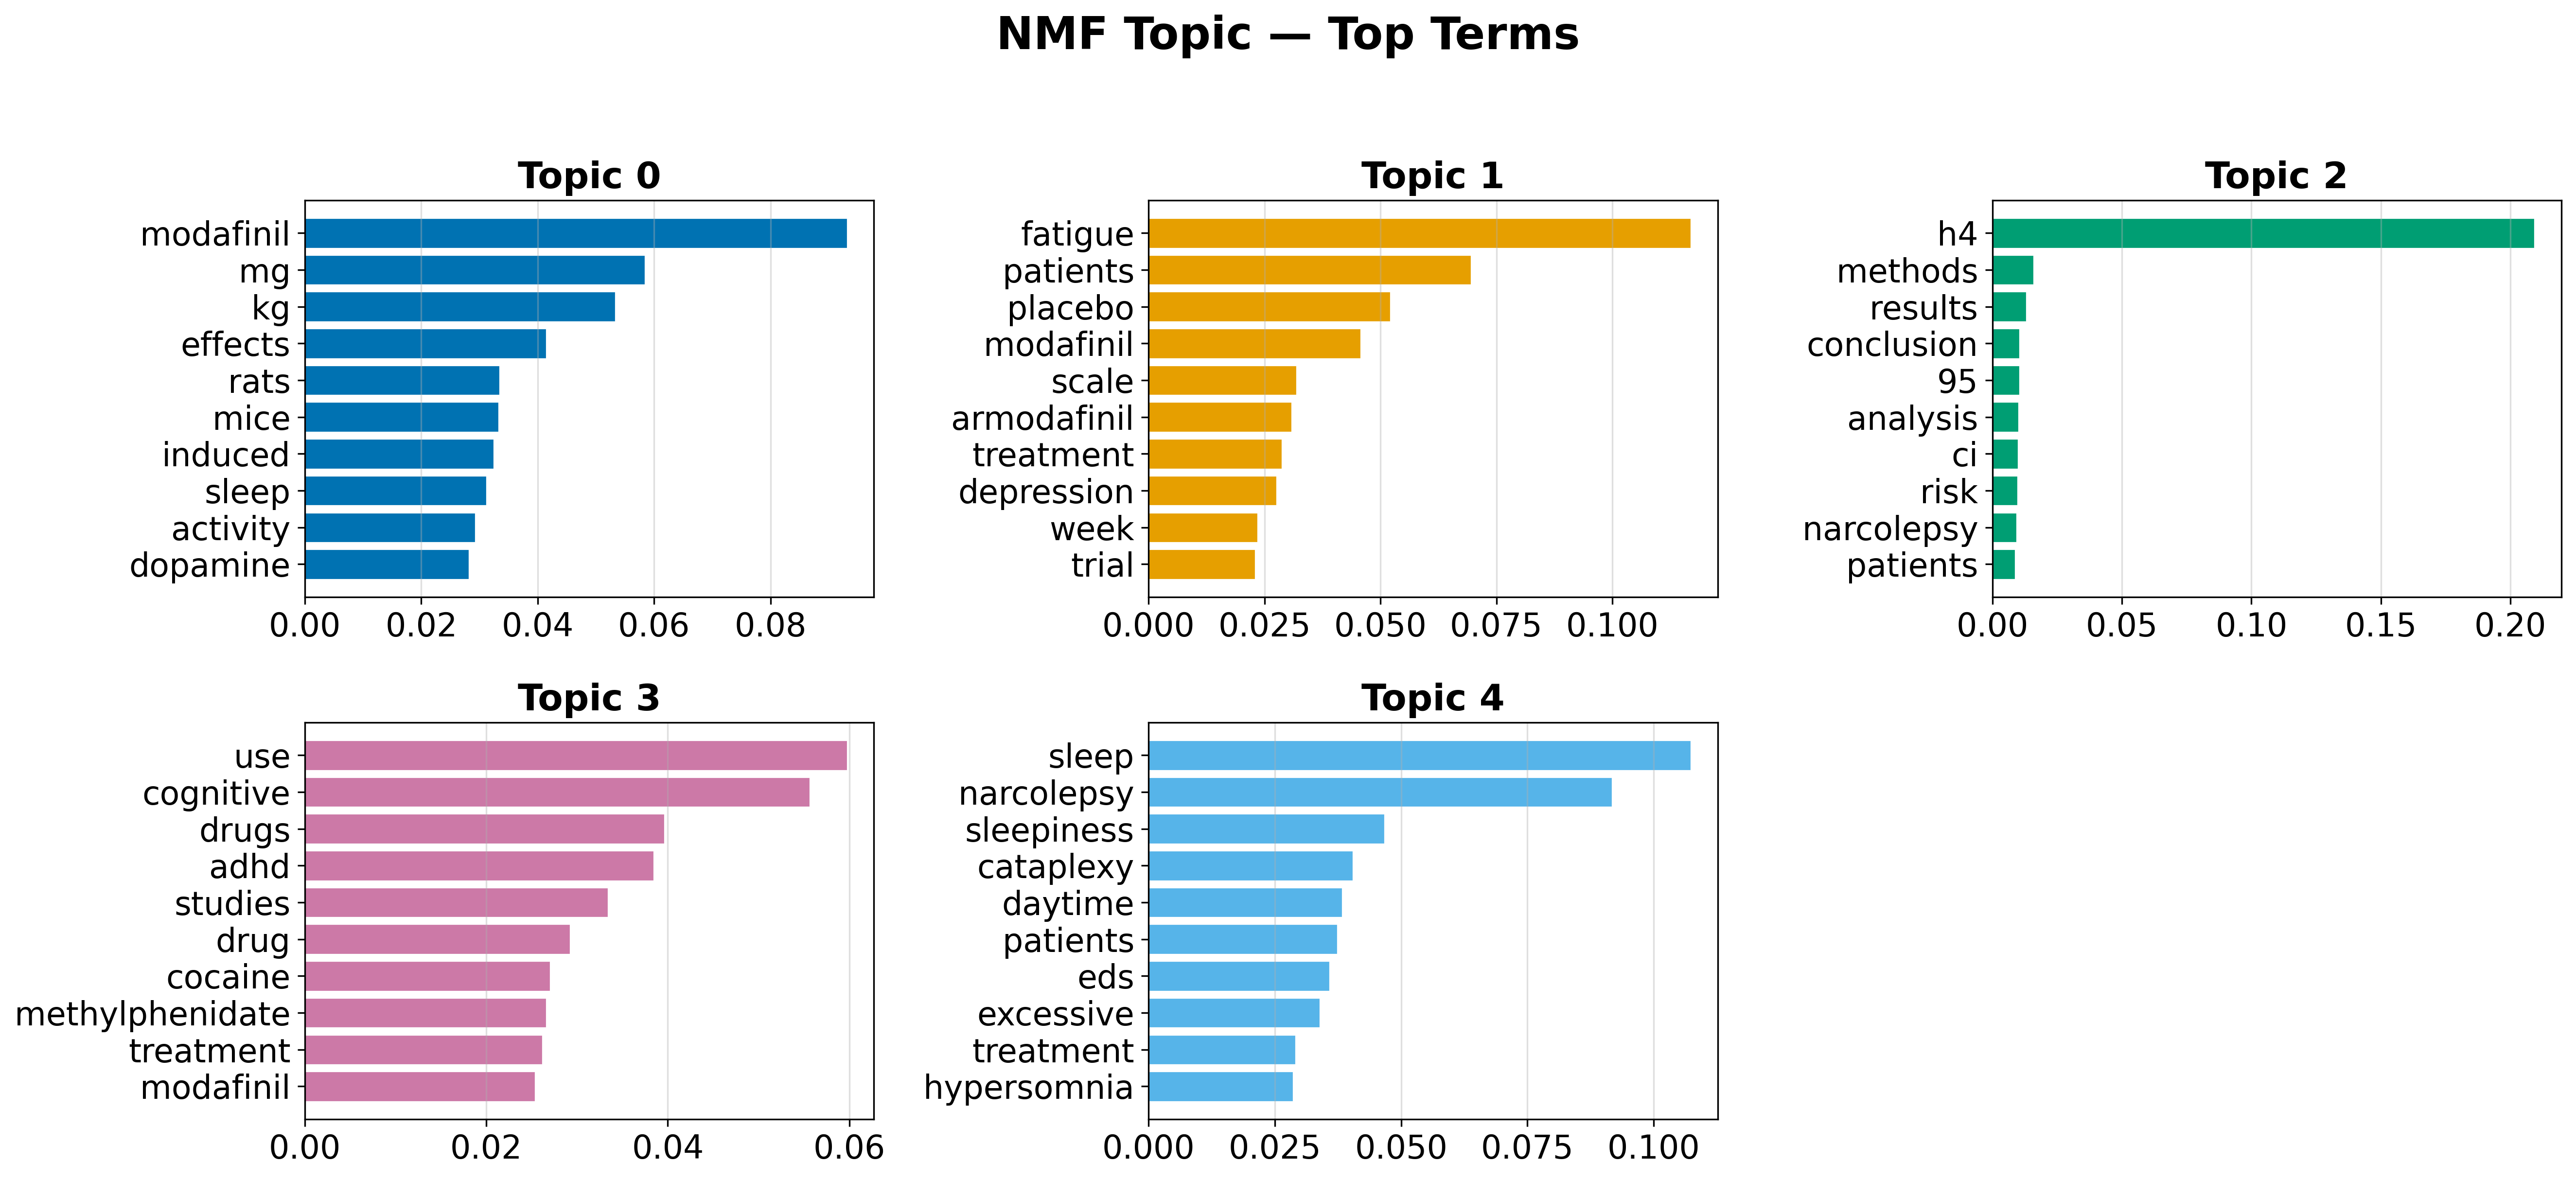
\includegraphics[keepaspectratio,alt={Topic-term bar charts for Modafinil. Each panel shows the top weighted terms for one of 5 NMF topics, with bar length proportional to the topic-term weight in the \textbackslash mathbf\{H\} matrix.}]{../figures/topic_term_bars.png}}\{\{\#fig:topic\_term\_bars\}\}
\end{frame}

\begin{frame}[allowframebreaks]{Document Embeddings}
\protect\phantomsection\label{document-embeddings}
Offline deterministic embeddings (TF-IDF followed by truncated SVD)
place every document in a shared 50-dimensional vector space. Embedding
the same text twice yields identical vectors, so the derived similarity
matrix, nearest-neighbour lists, clusters, and two-dimensional
projection are all reproducible.

\pandocbounded{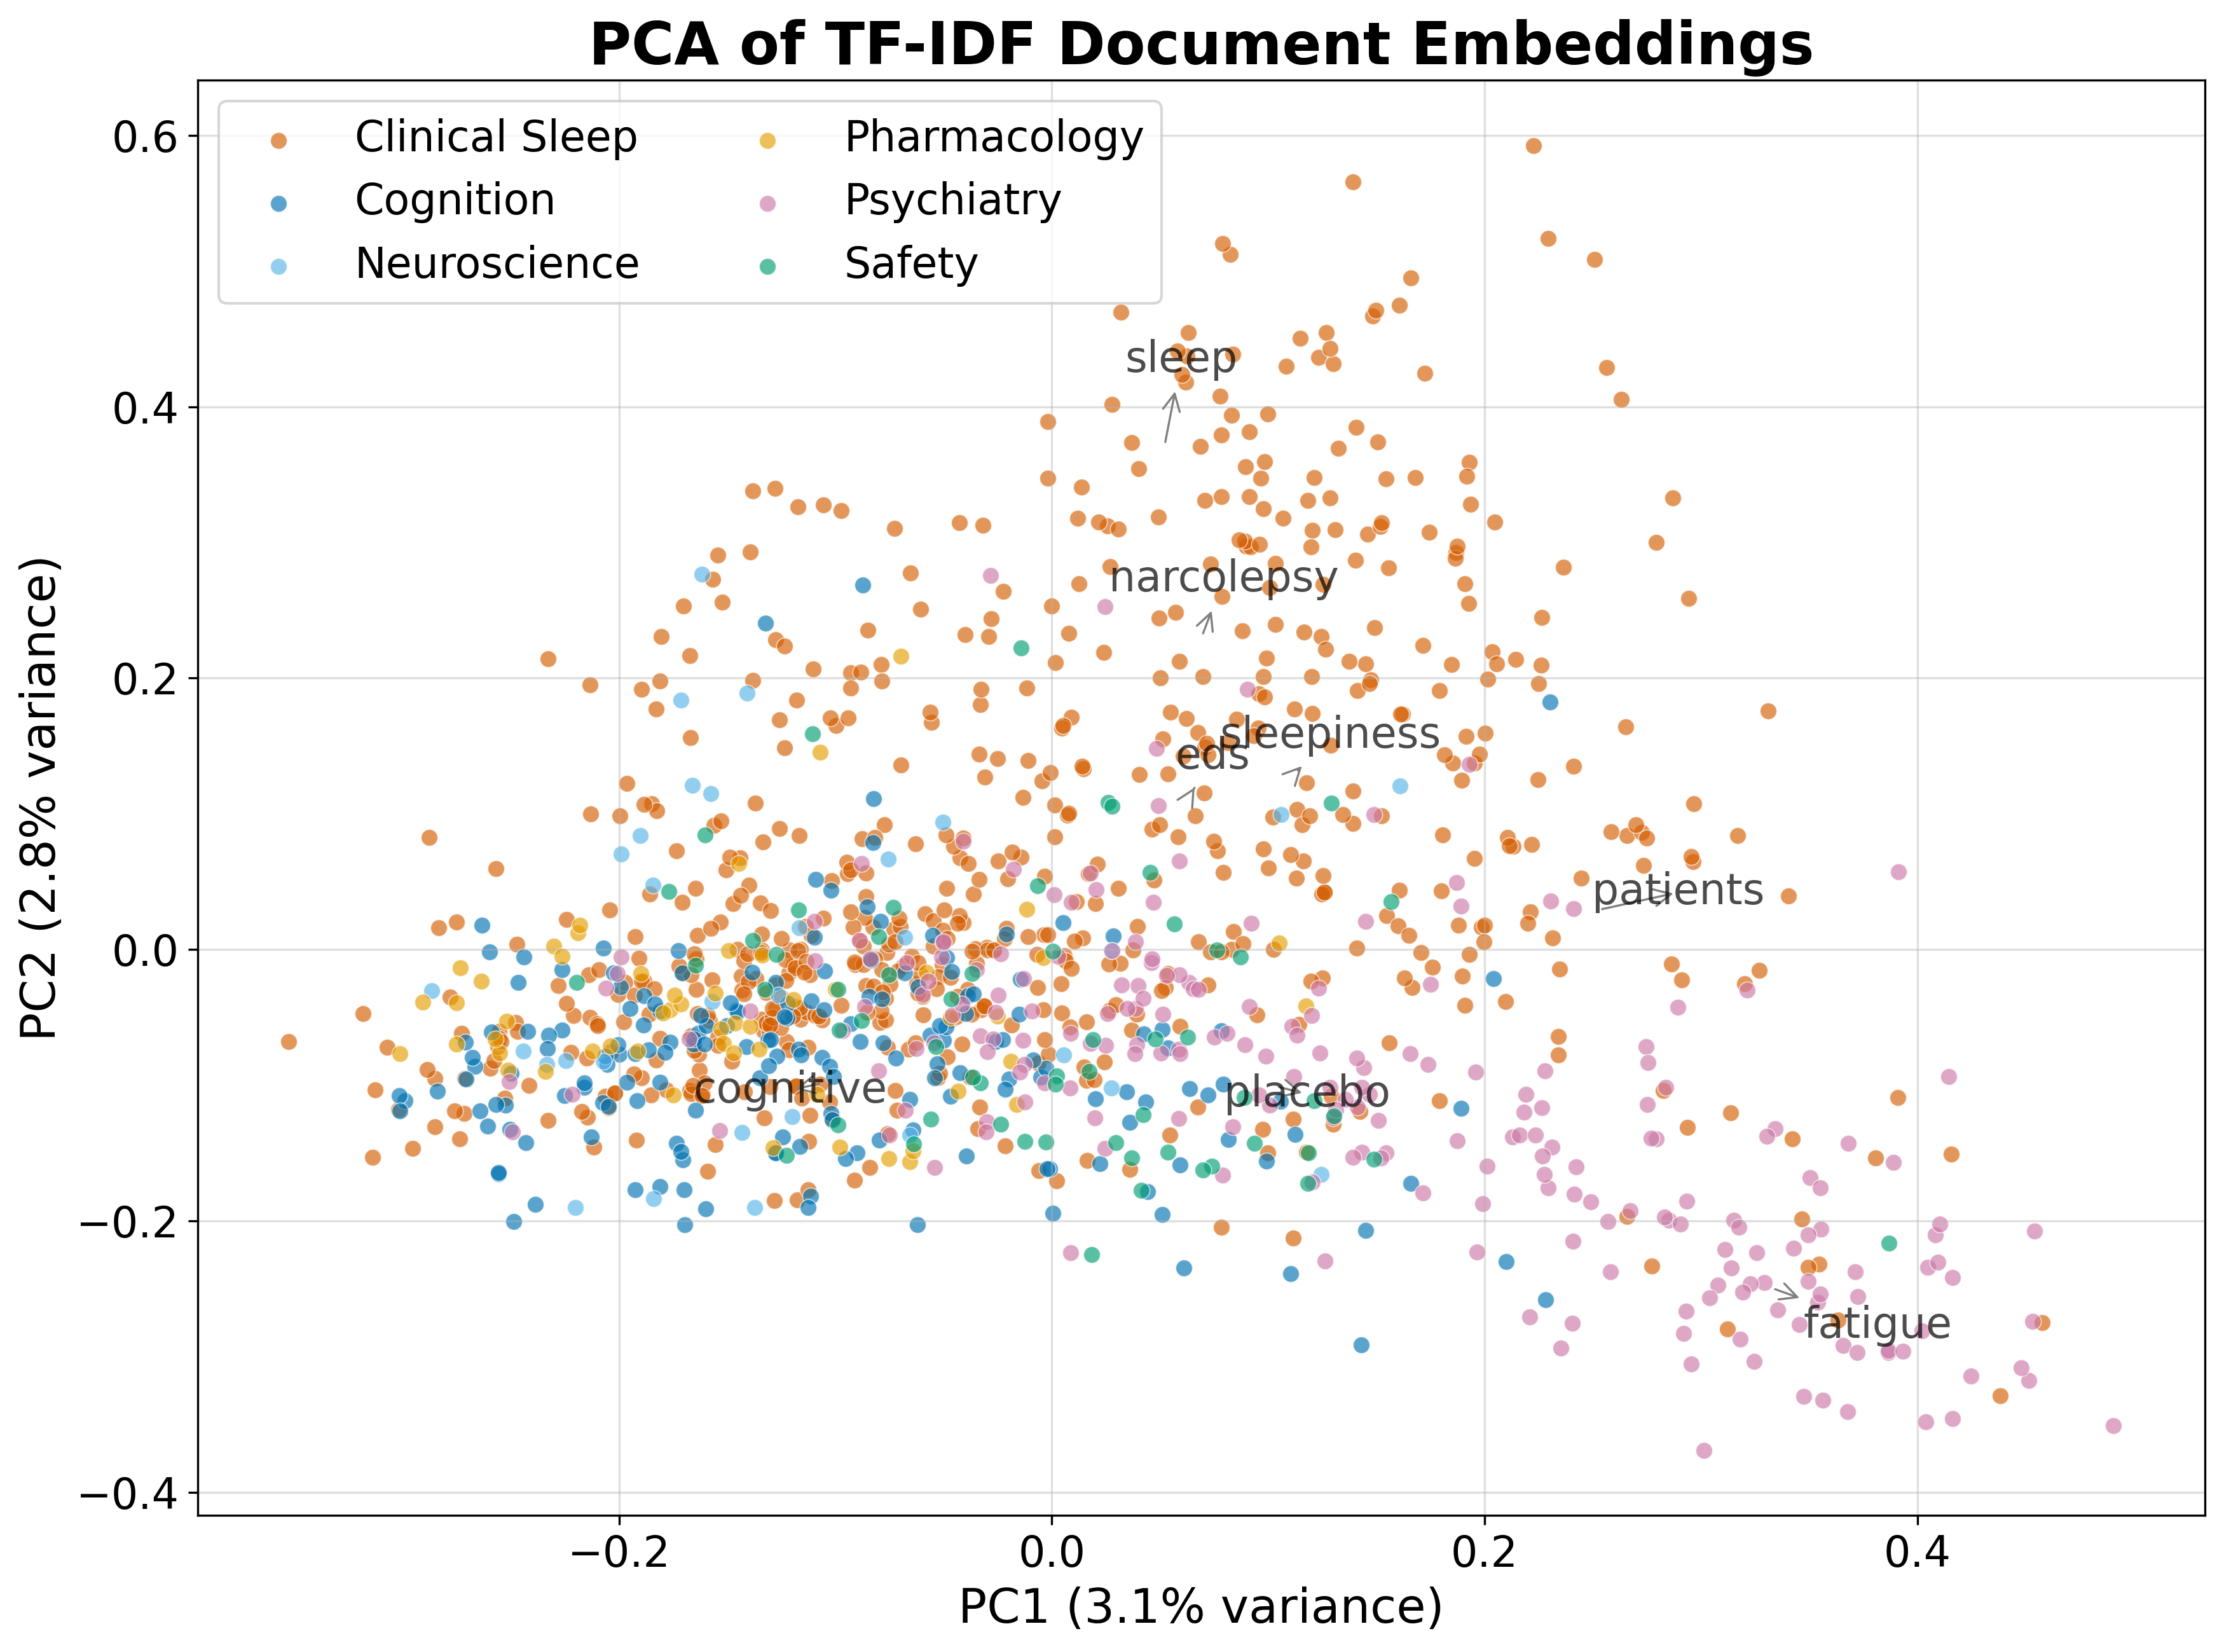
\includegraphics[keepaspectratio,alt={PCA projection of document embeddings for Modafinil. Each point represents one document projected onto the first two principal components of the TF-IDF/SVD embedding. Colours indicate subfield assignment, showing how the topical geography relates to the keyword taxonomy.}]{../figures/pca_embeddings.png}}\{\{\#fig:pca\_embeddings\}\}

\pandocbounded{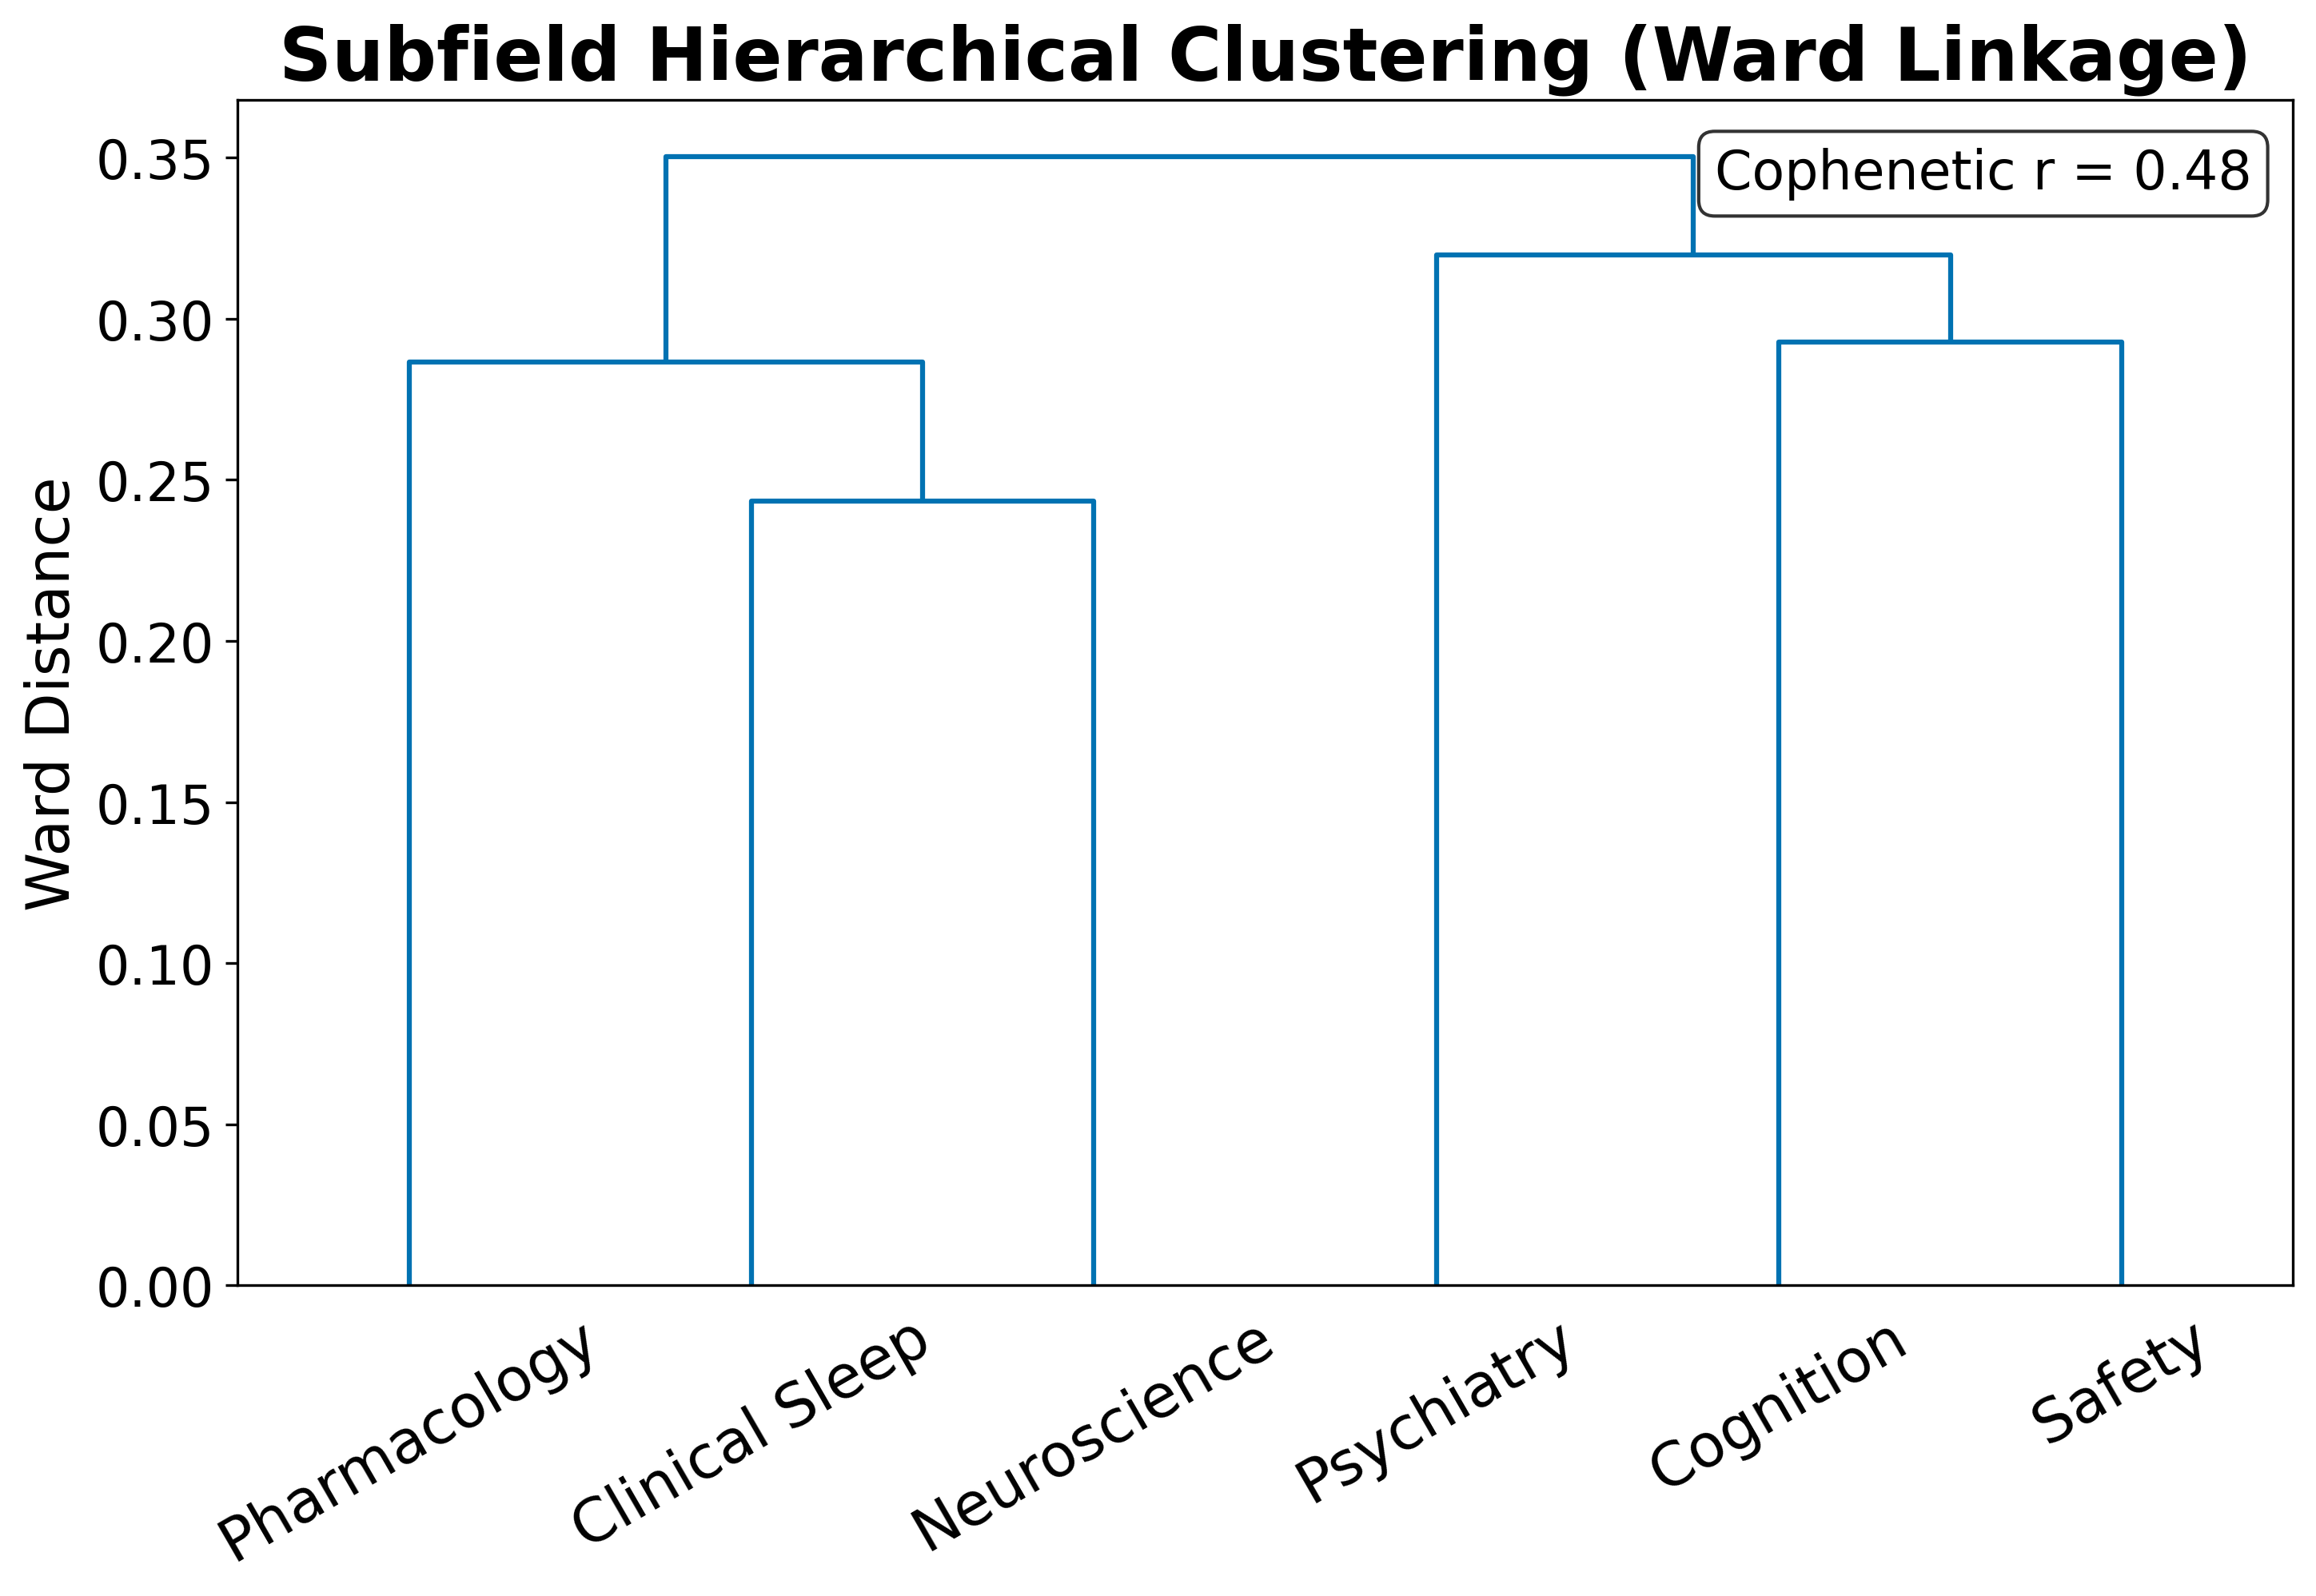
\includegraphics[keepaspectratio,alt={Hierarchical clustering dendrogram of document embeddings. The tree shows the similarity structure of the corpus: documents that join low in the tree are semantically similar, while high-level splits separate the major topical clusters.}]{../figures/dendrogram.png}}\{\{\#fig:dendrogram\}\}
\end{frame}

\begin{frame}[allowframebreaks]{Term Analysis}
\protect\phantomsection\label{term-analysis}
The TF-IDF term heatmap reveals which terms discriminate between
subfields: terms with high between-subfield variance (rather than high
global mean) are selected for display.

\pandocbounded{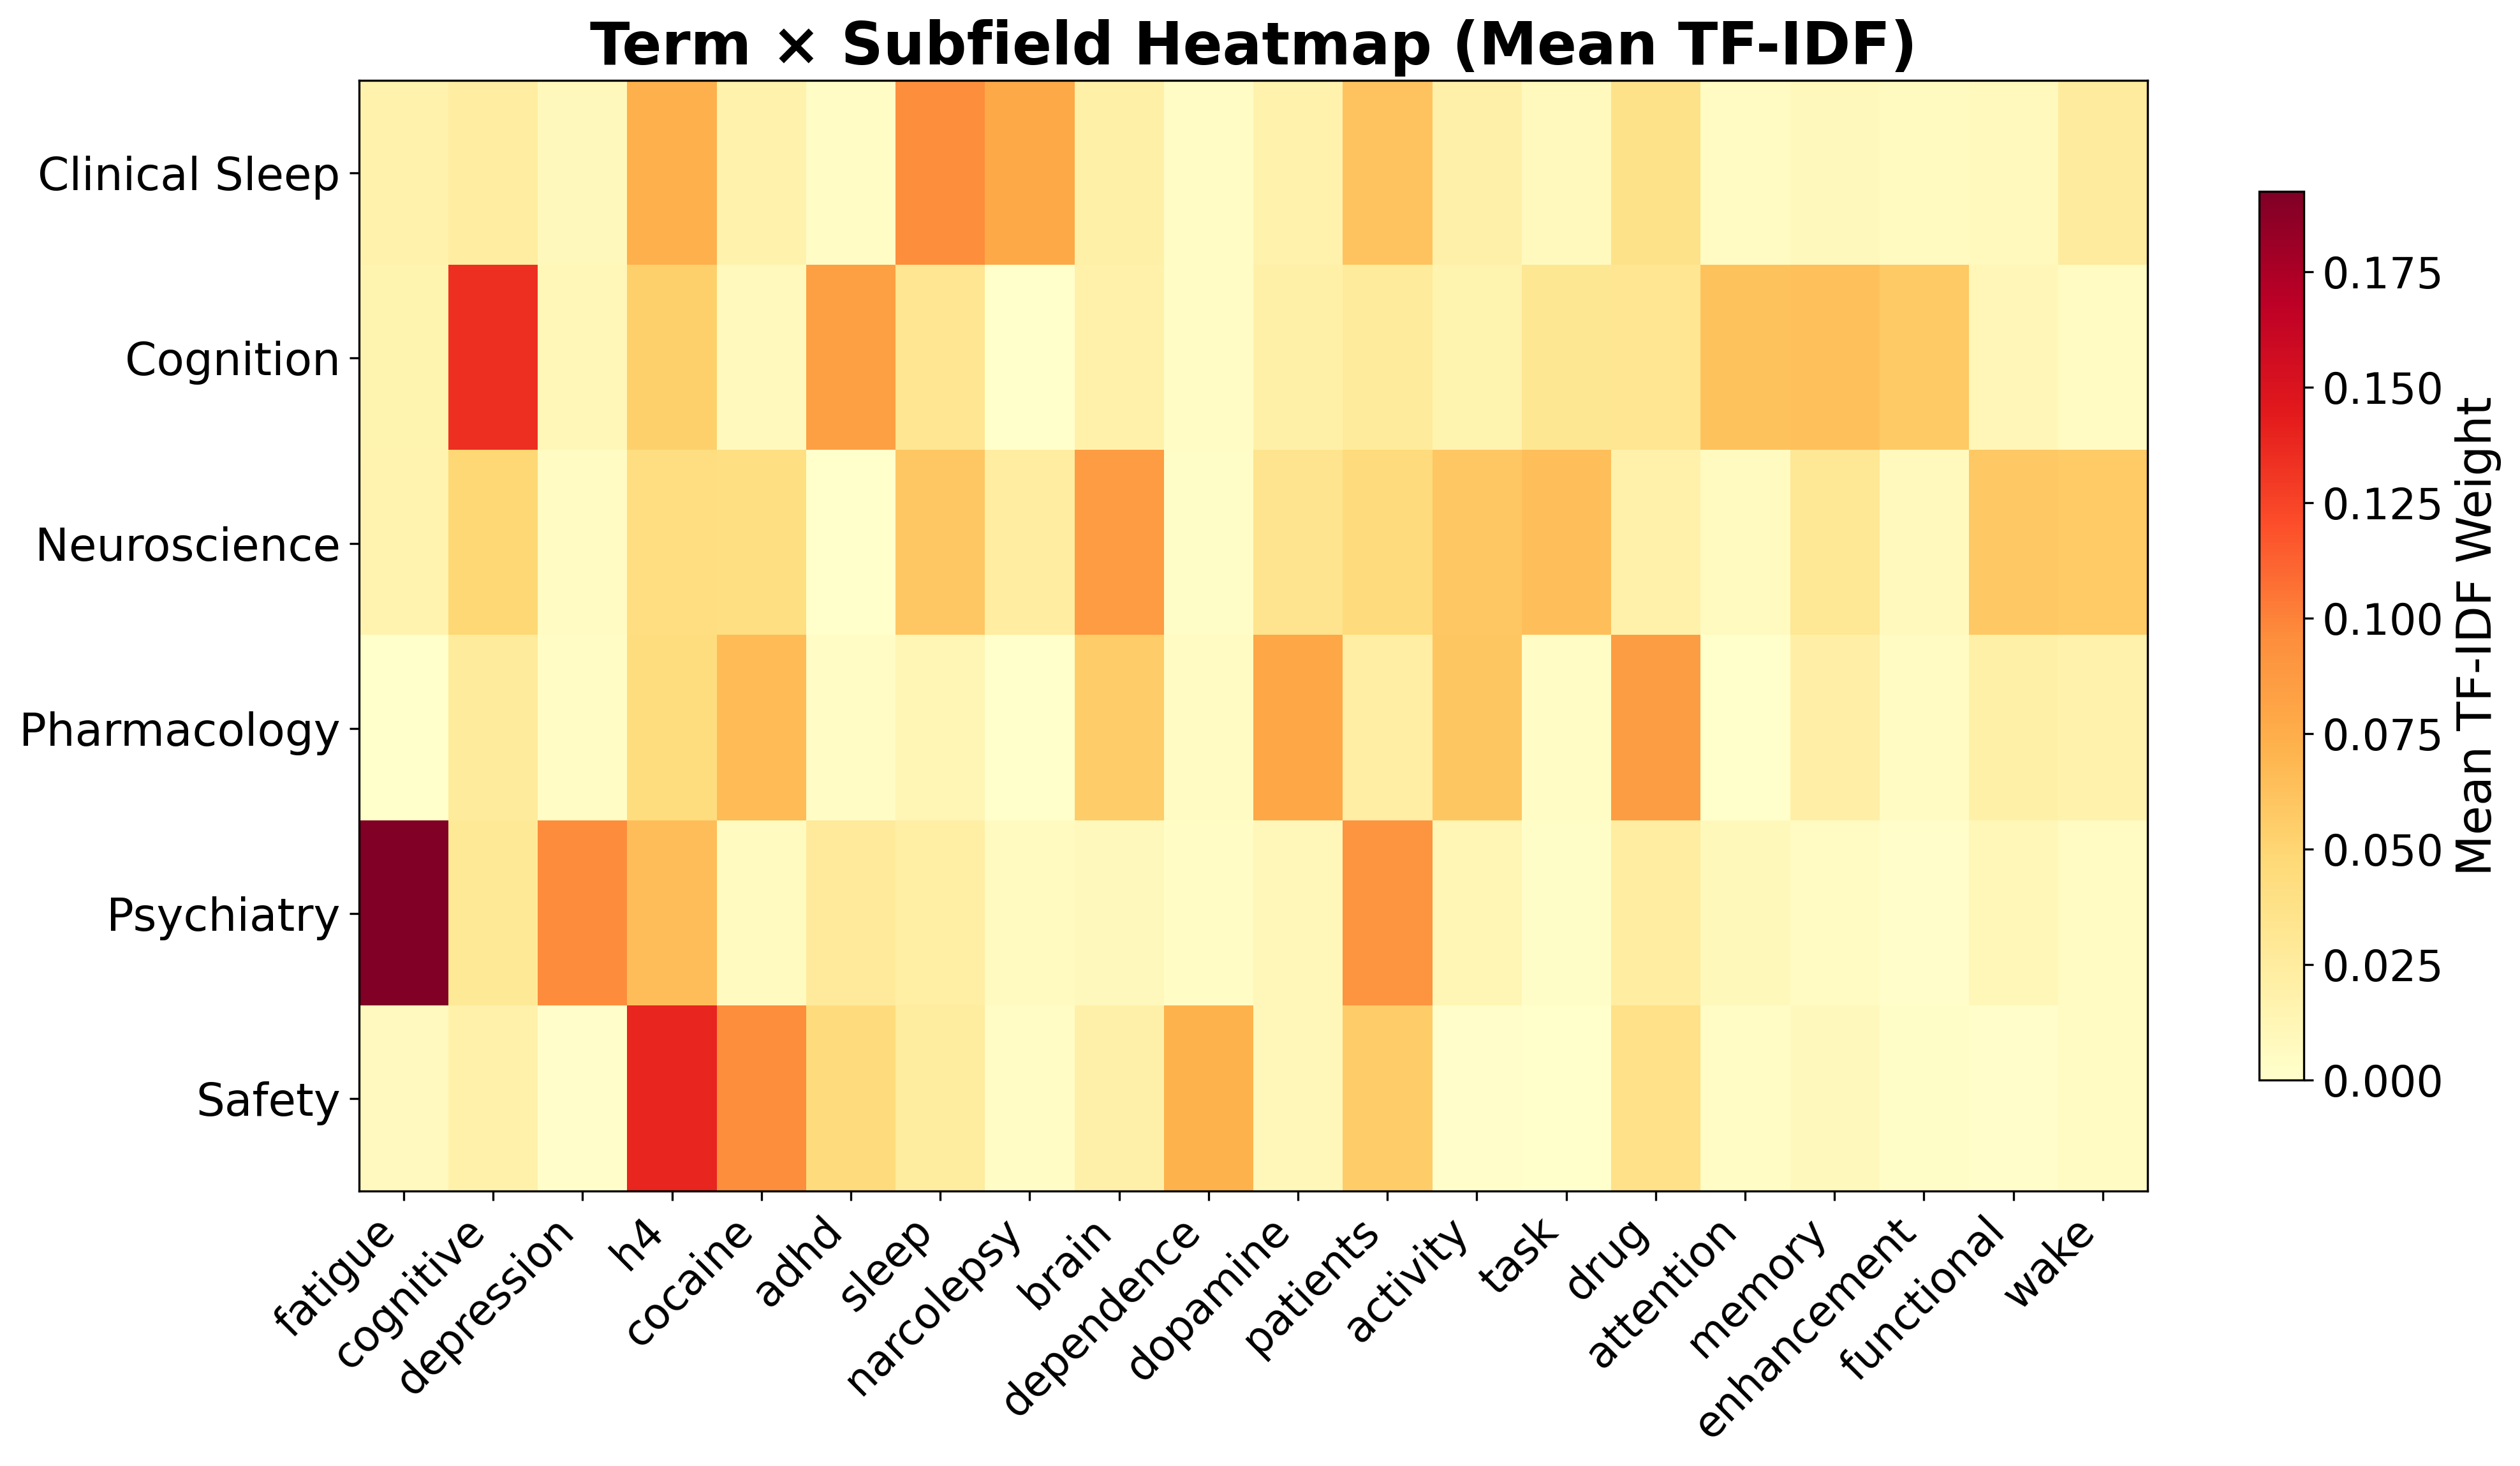
\includegraphics[keepaspectratio,alt={Term heatmap for Modafinil. Each cell shows the mean TF-IDF weight of a term within a subfield. Terms are selected by between-subfield variance to highlight discriminative vocabulary rather than globally frequent terms.}]{../figures/term_heatmap.png}}\{\{\#fig:term\_heatmap\}\}
\end{frame}

\begin{frame}[allowframebreaks]{Named Entity Analysis}
\protect\phantomsection\label{named-entity-analysis}
Named entity extraction over the 1277 abstracts identified 30 unique
entities. The most frequent entities reflect the clinical and
pharmacological vocabulary of the modafinil literature.

\textbf{Table 4. Top named entities in abstracts.}

{\def\LTcaptype{none} % do not increment counter
\begin{longtable}[]{@{}ll@{}}
\toprule\noalign{}
Entity & Frequency \\
\midrule\noalign{}
\endhead
ADHD & 338 \\
CI & 315 \\
EDS & 258 \\
OSA & 236 \\
MOD & 158 \\
RESULTS & 152 \\
DAT & 133 \\
MS & 132 \\
CONCLUSIONS & 130 \\
ESS & 127 \\
SD & 113 \\
METHODS & 102 \\
CE & 101 \\
MD & 97 \\
IH & 88 \\
\bottomrule\noalign{}
\end{longtable}
}

\pandocbounded{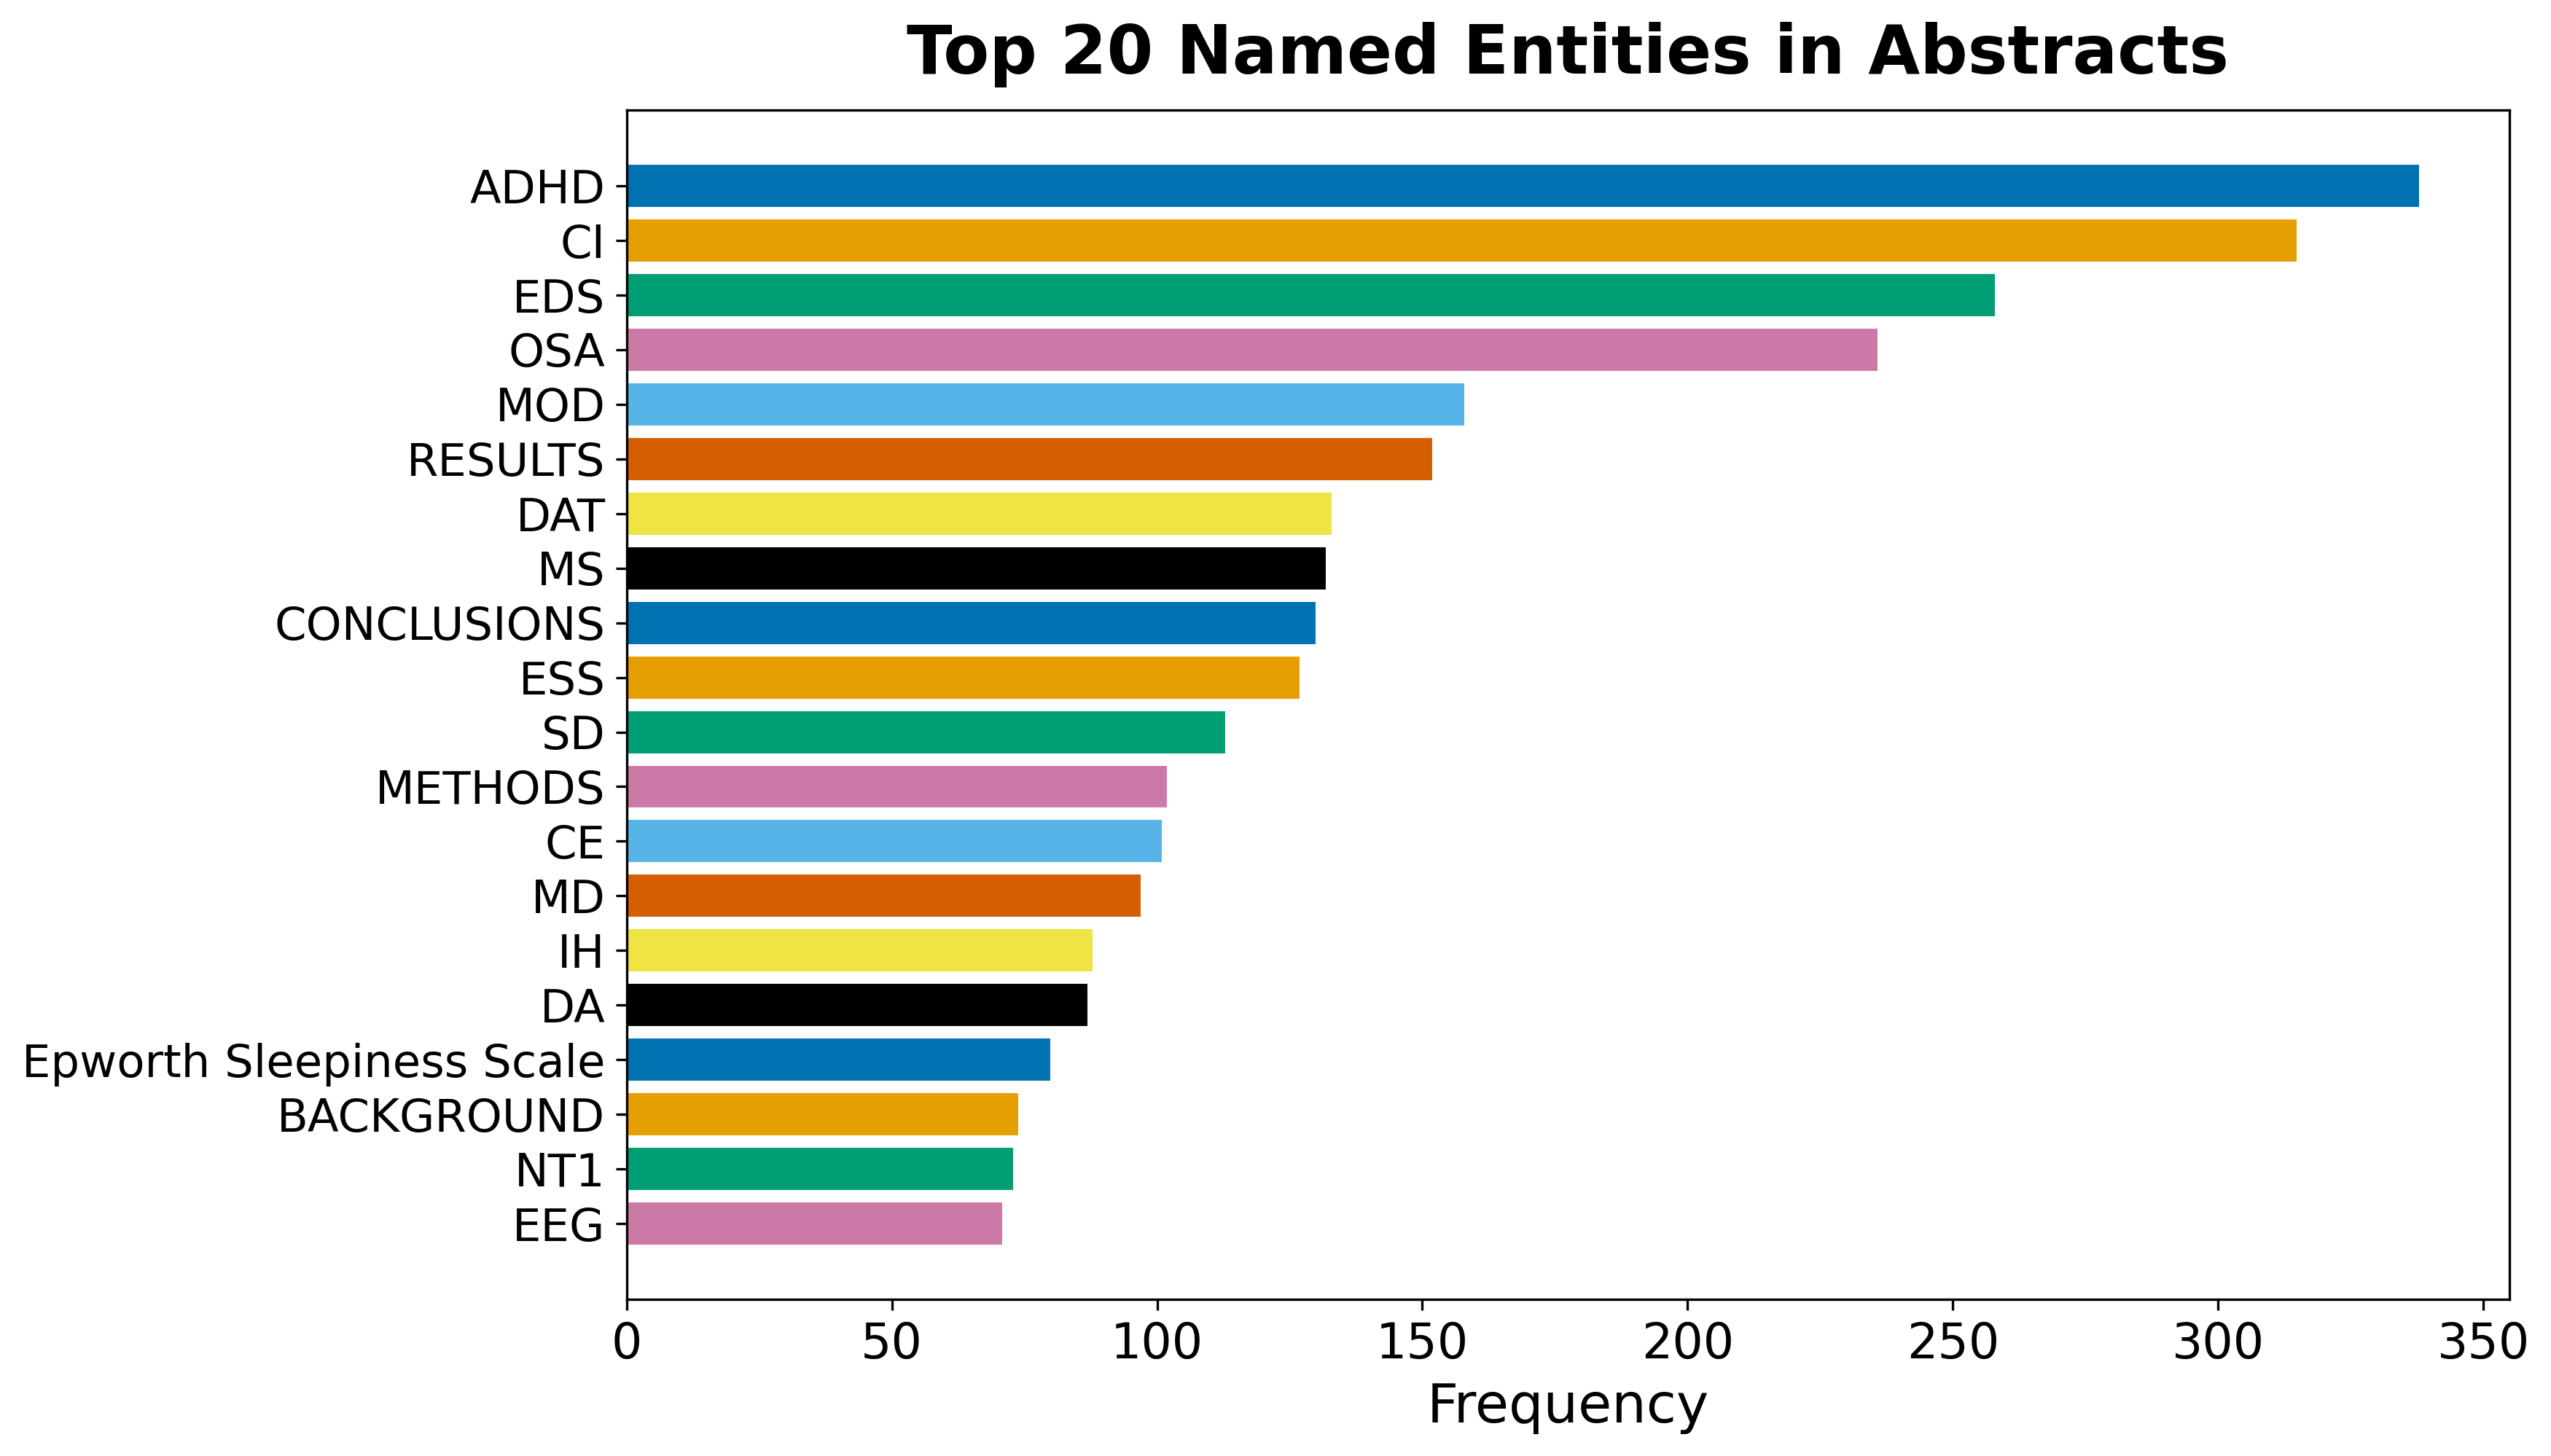
\includegraphics[keepaspectratio,alt={Top named entities for Modafinil. The horizontal bar chart shows the 20 most frequently extracted named entities from abstracts, revealing the dominant drugs, conditions, and concepts in the literature.}]{../figures/entity_bar_chart.png}}\{\{\#fig:entity\_bar\_chart\}\}

\textbf{Table 5. Top keyphrases by TF-IDF score.}

{\def\LTcaptype{none} % do not increment counter
\begin{longtable}[]{@{}ll@{}}
\toprule\noalign{}
Keyphrase & Score \\
\midrule\noalign{}
\endhead
available & 0.3333 \\
abstract & 0.3333 \\
abstract available & 0.3333 \\
content & 0.1053 \\
access & 0.1053 \\
md & 0.0870 \\
jama & 0.0826 \\
cleveland & 0.0763 \\
modafinil & 0.0741 \\
depression & 0.0741 \\
substance & 0.0694 \\
drug & 0.0667 \\
conditions & 0.0667 \\
continuous & 0.0667 \\
continuous flow & 0.0667 \\
\bottomrule\noalign{}
\end{longtable}
}
\end{frame}

\begin{frame}[allowframebreaks]{Embedding Similarity and Clustering}
\protect\phantomsection\label{embedding-similarity-and-clustering}
The TF-IDF/SVD embeddings place every document in a 50-dimensional
vector space. K-means clustering with \(k = 5\) clusters partitions the
corpus into topically coherent groups. The top similar document pairs,
ranked by cosine similarity, reveal the most closely related works in
the corpus.

\textbf{Table 6. Top 10 most similar document pairs.}

{\def\LTcaptype{none} % do not increment counter
\begin{longtable}[]{@{}
  >{\raggedright\arraybackslash}p{(\linewidth - 4\tabcolsep) * \real{0.3333}}
  >{\raggedright\arraybackslash}p{(\linewidth - 4\tabcolsep) * \real{0.3333}}
  >{\raggedright\arraybackslash}p{(\linewidth - 4\tabcolsep) * \real{0.3333}}@{}}
\toprule\noalign{}
\begin{minipage}[b]{\linewidth}\raggedright
Paper A
\end{minipage} & \begin{minipage}[b]{\linewidth}\raggedright
Paper B
\end{minipage} & \begin{minipage}[b]{\linewidth}\raggedright
Similarity
\end{minipage} \\
\midrule\noalign{}
\endhead
doi:10.1176/appi.ajp.163.12.21 & doi:10.1176/ajp.2006.163.12.21 &
1.0000 \\
doi:10.1176/ajp.2006.163.12.21 & doi:10.1176/appi.ajp.163.12.21 &
1.0000 \\
doi:10.1197/j.aem.2005.08.013 & doi:10.1111/j.1553-2712.2006.t &
1.0000 \\
doi:10.1345/aph.1h302 & doi:10.1136/bcr.08.2011.4652 & 0.9687 \\
doi:10.4088/jcp.09m05900gry & doi:10.1186/s40345-015-0034-0 & 0.9628 \\
doi:10.1016/s2215-0366(18)3026 & doi:10.1016/s2215-0366(25)0006 &
0.9621 \\
doi:10.1345/aph.1h302 & doi:10.1017/neu.2023.6 & 0.9598 \\
doi:10.1111/j.1365-2869.2008.0 & doi:10.3109/07420528.2011.6352 &
0.9538 \\
doi:10.1513/annalsats.202006-6 & doi:10.3760/cma.j.cn112147-202 &
0.9532 \\
doi:10.1345/aph.1h302 & doi:10.1192/bjo.2024.75 & 0.9517 \\
\bottomrule\noalign{}
\end{longtable}
}

\pandocbounded{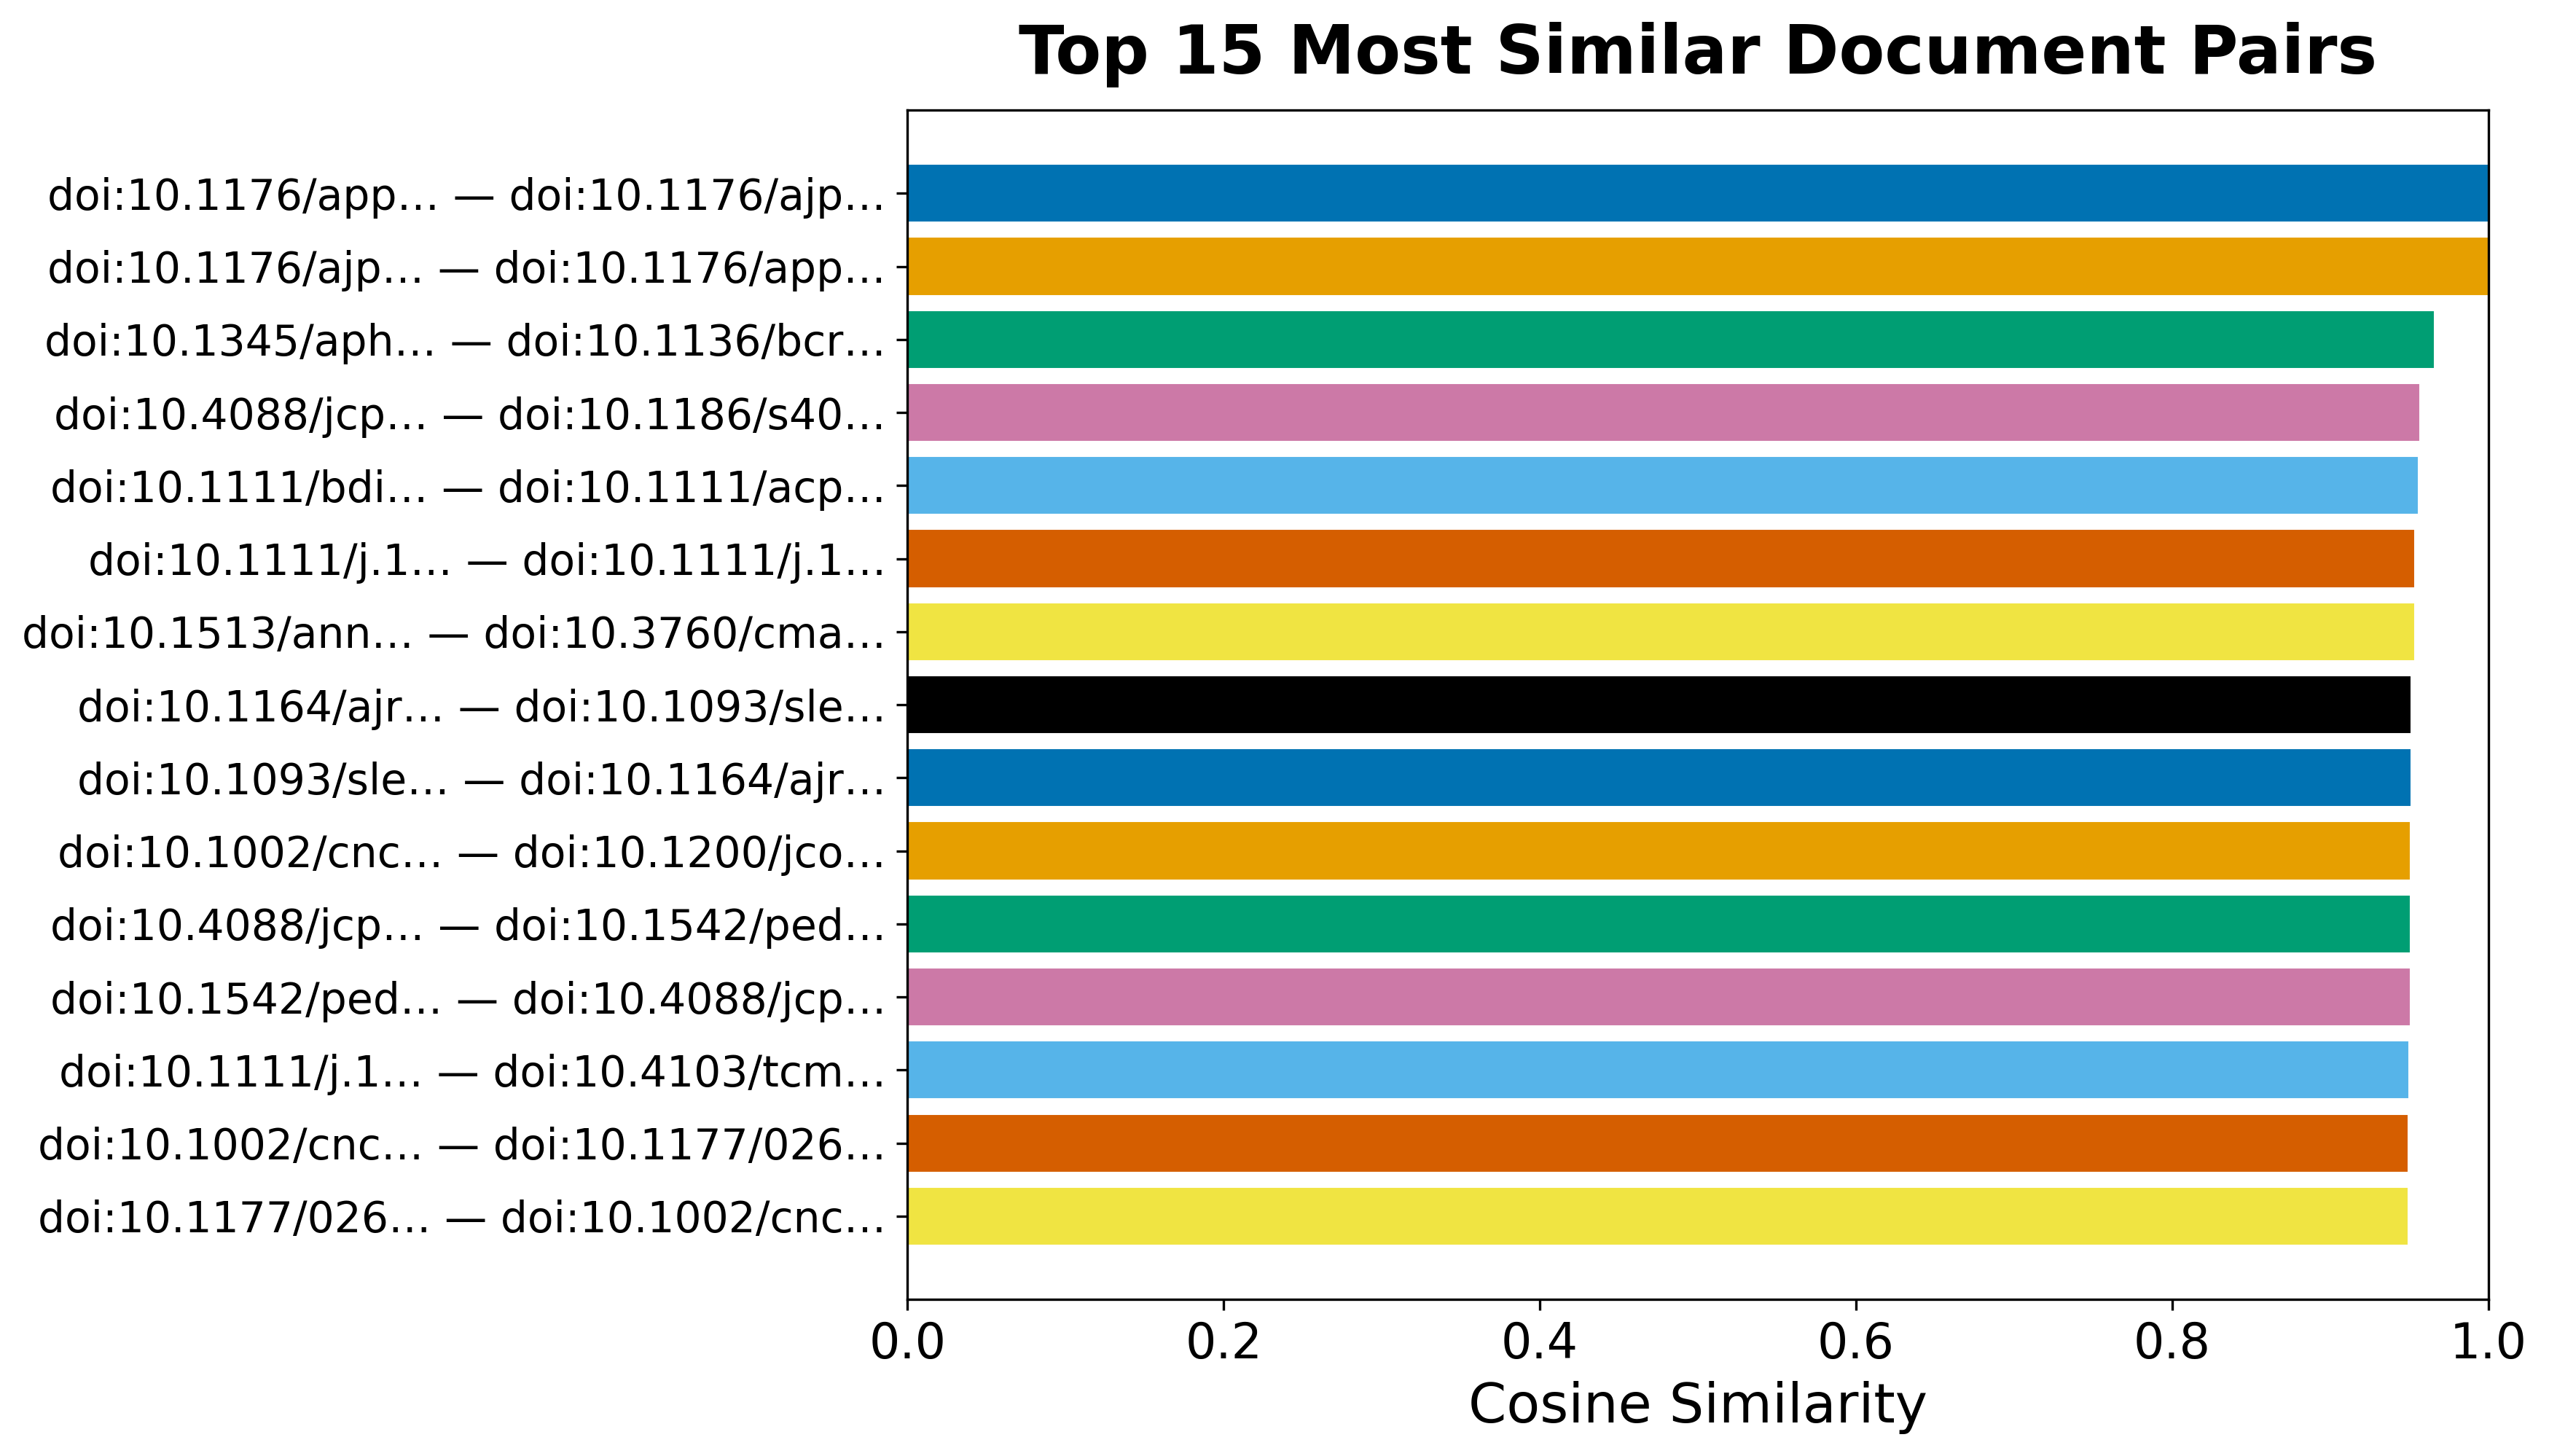
\includegraphics[keepaspectratio,alt={Document similarity for Modafinil. The horizontal bar chart shows the 15 most similar document pairs ranked by cosine similarity of their TF-IDF/SVD embeddings. High-similarity pairs share topical and lexical content.}]{../figures/similarity_heatmap.png}}\{\{\#fig:similarity\_heatmap\}\}

\pandocbounded{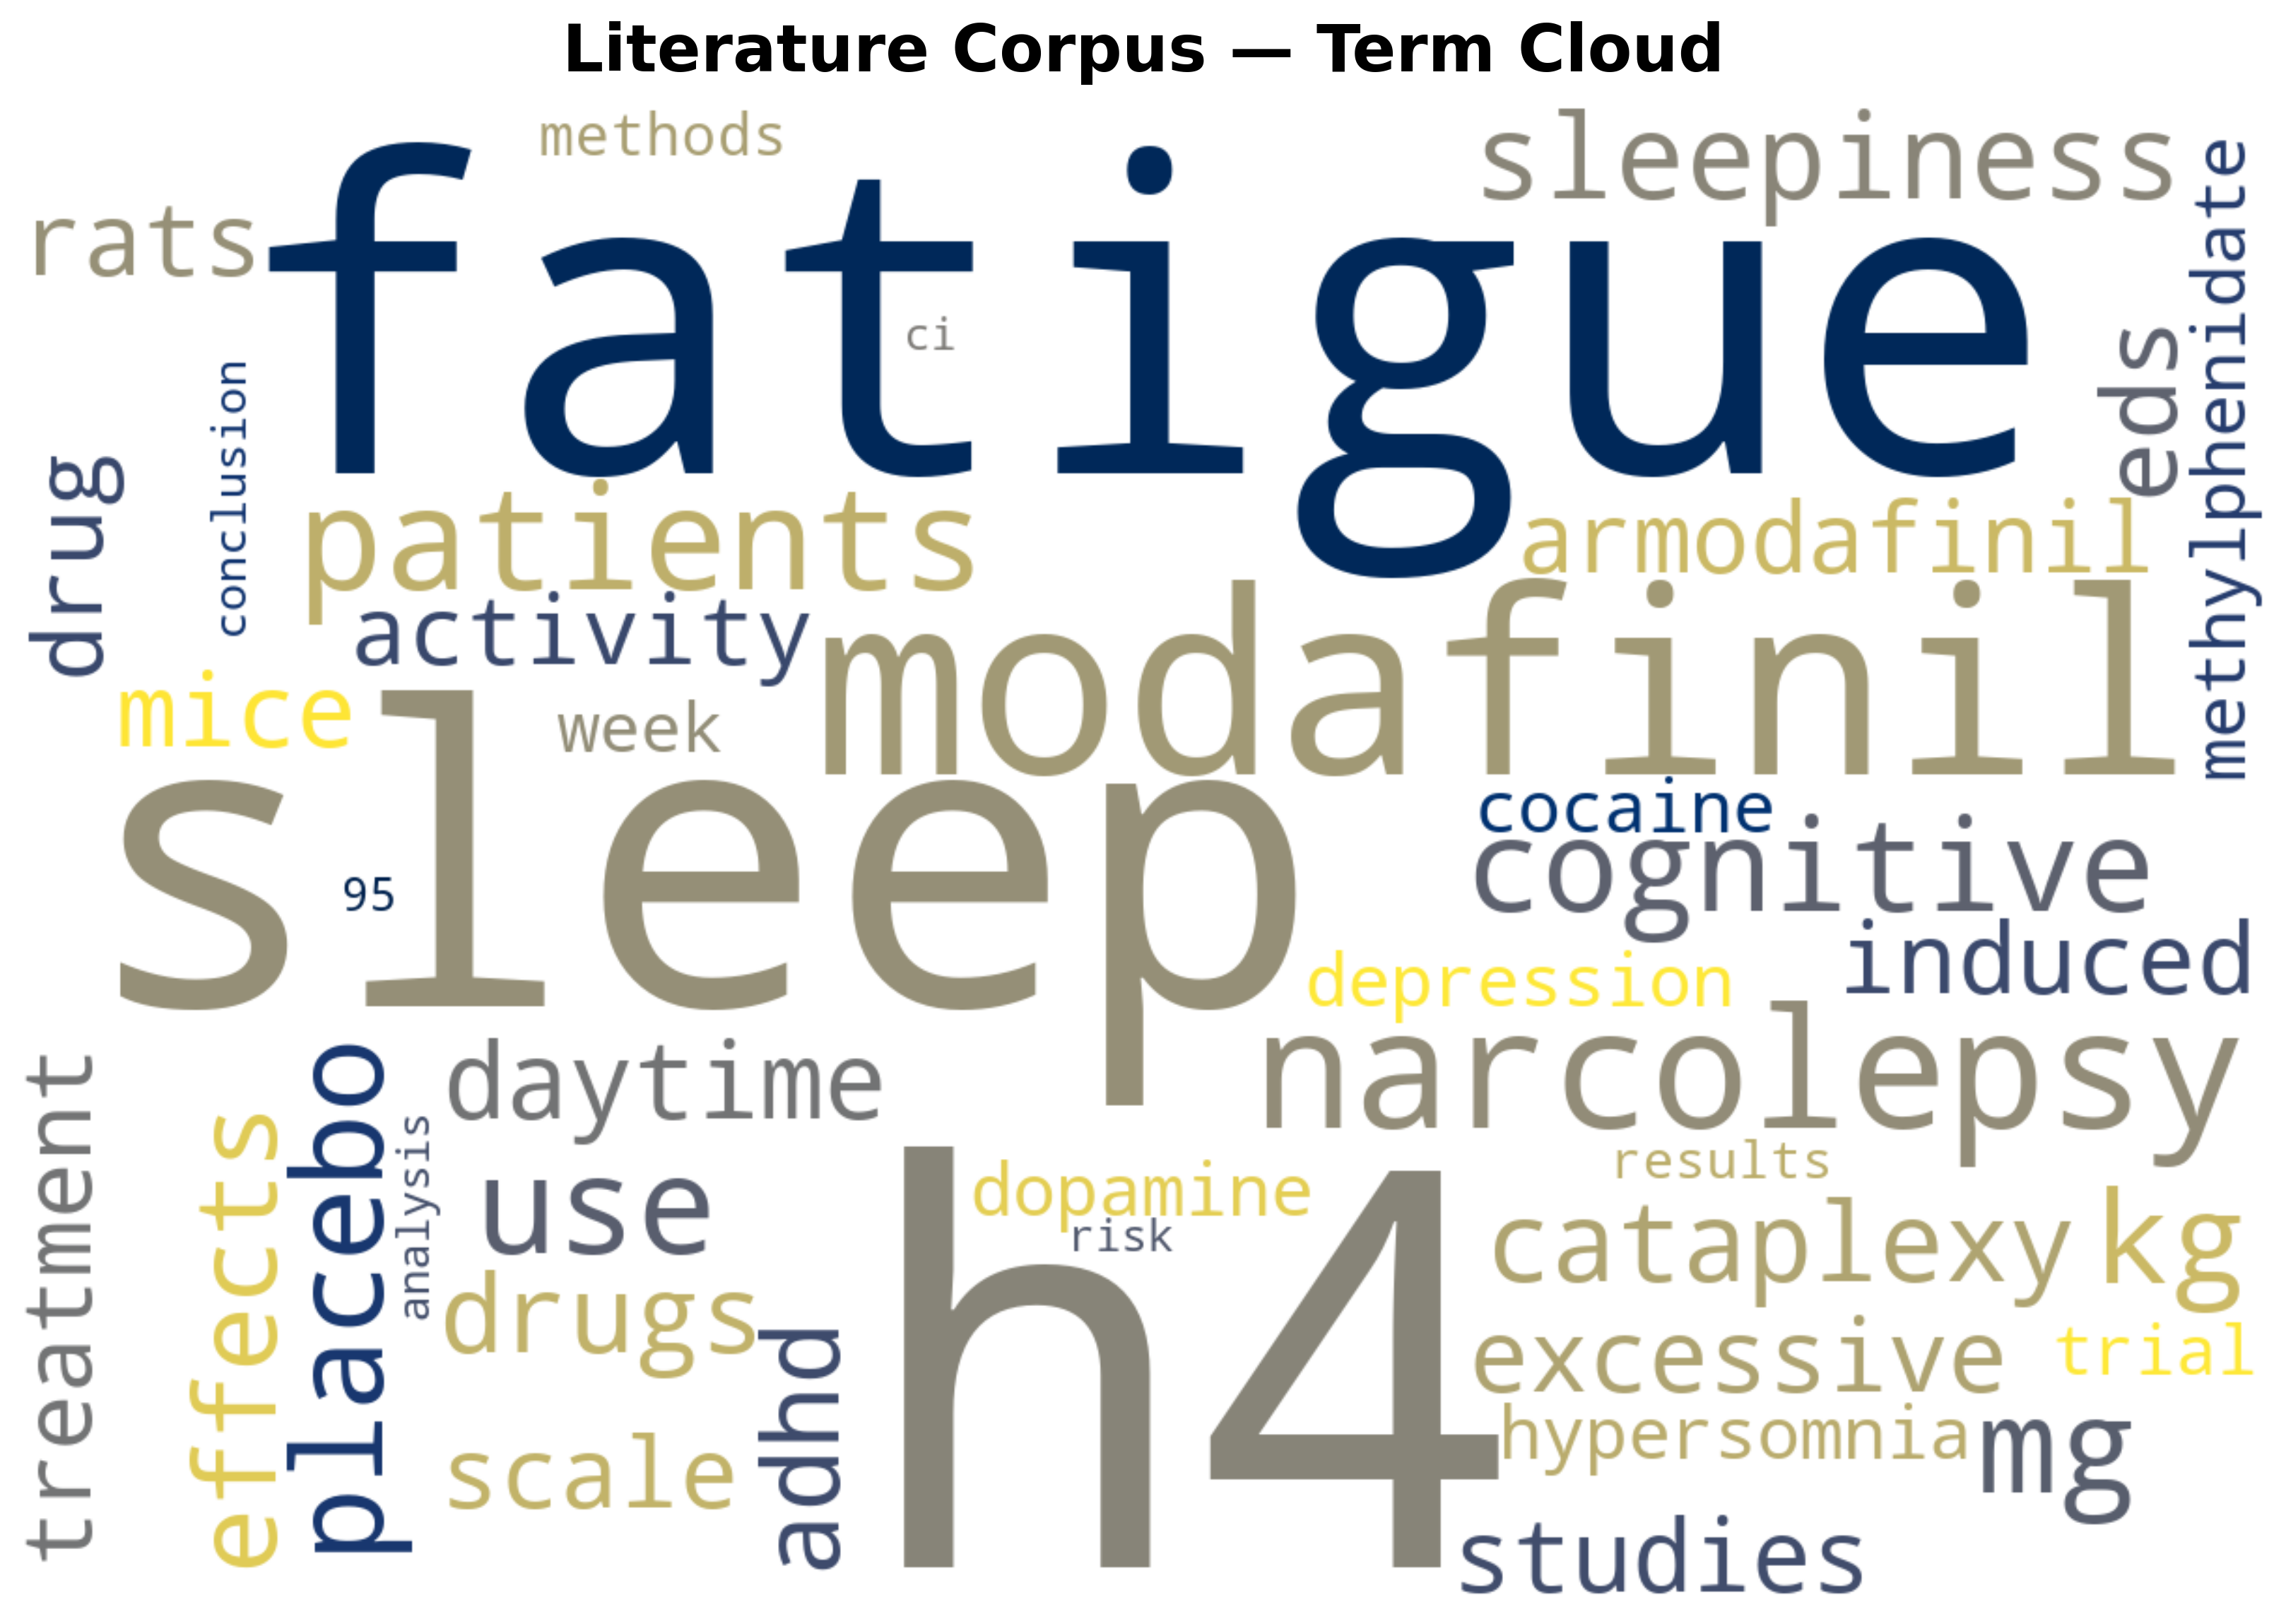
\includegraphics[keepaspectratio,alt={Term cloud for Modafinil. Term sizes are proportional to their TF-IDF weights across the corpus, providing a visual summary of the dominant vocabulary.}]{../figures/word_cloud.png}}\{\{\#fig:word\_cloud\}\}

\pandocbounded{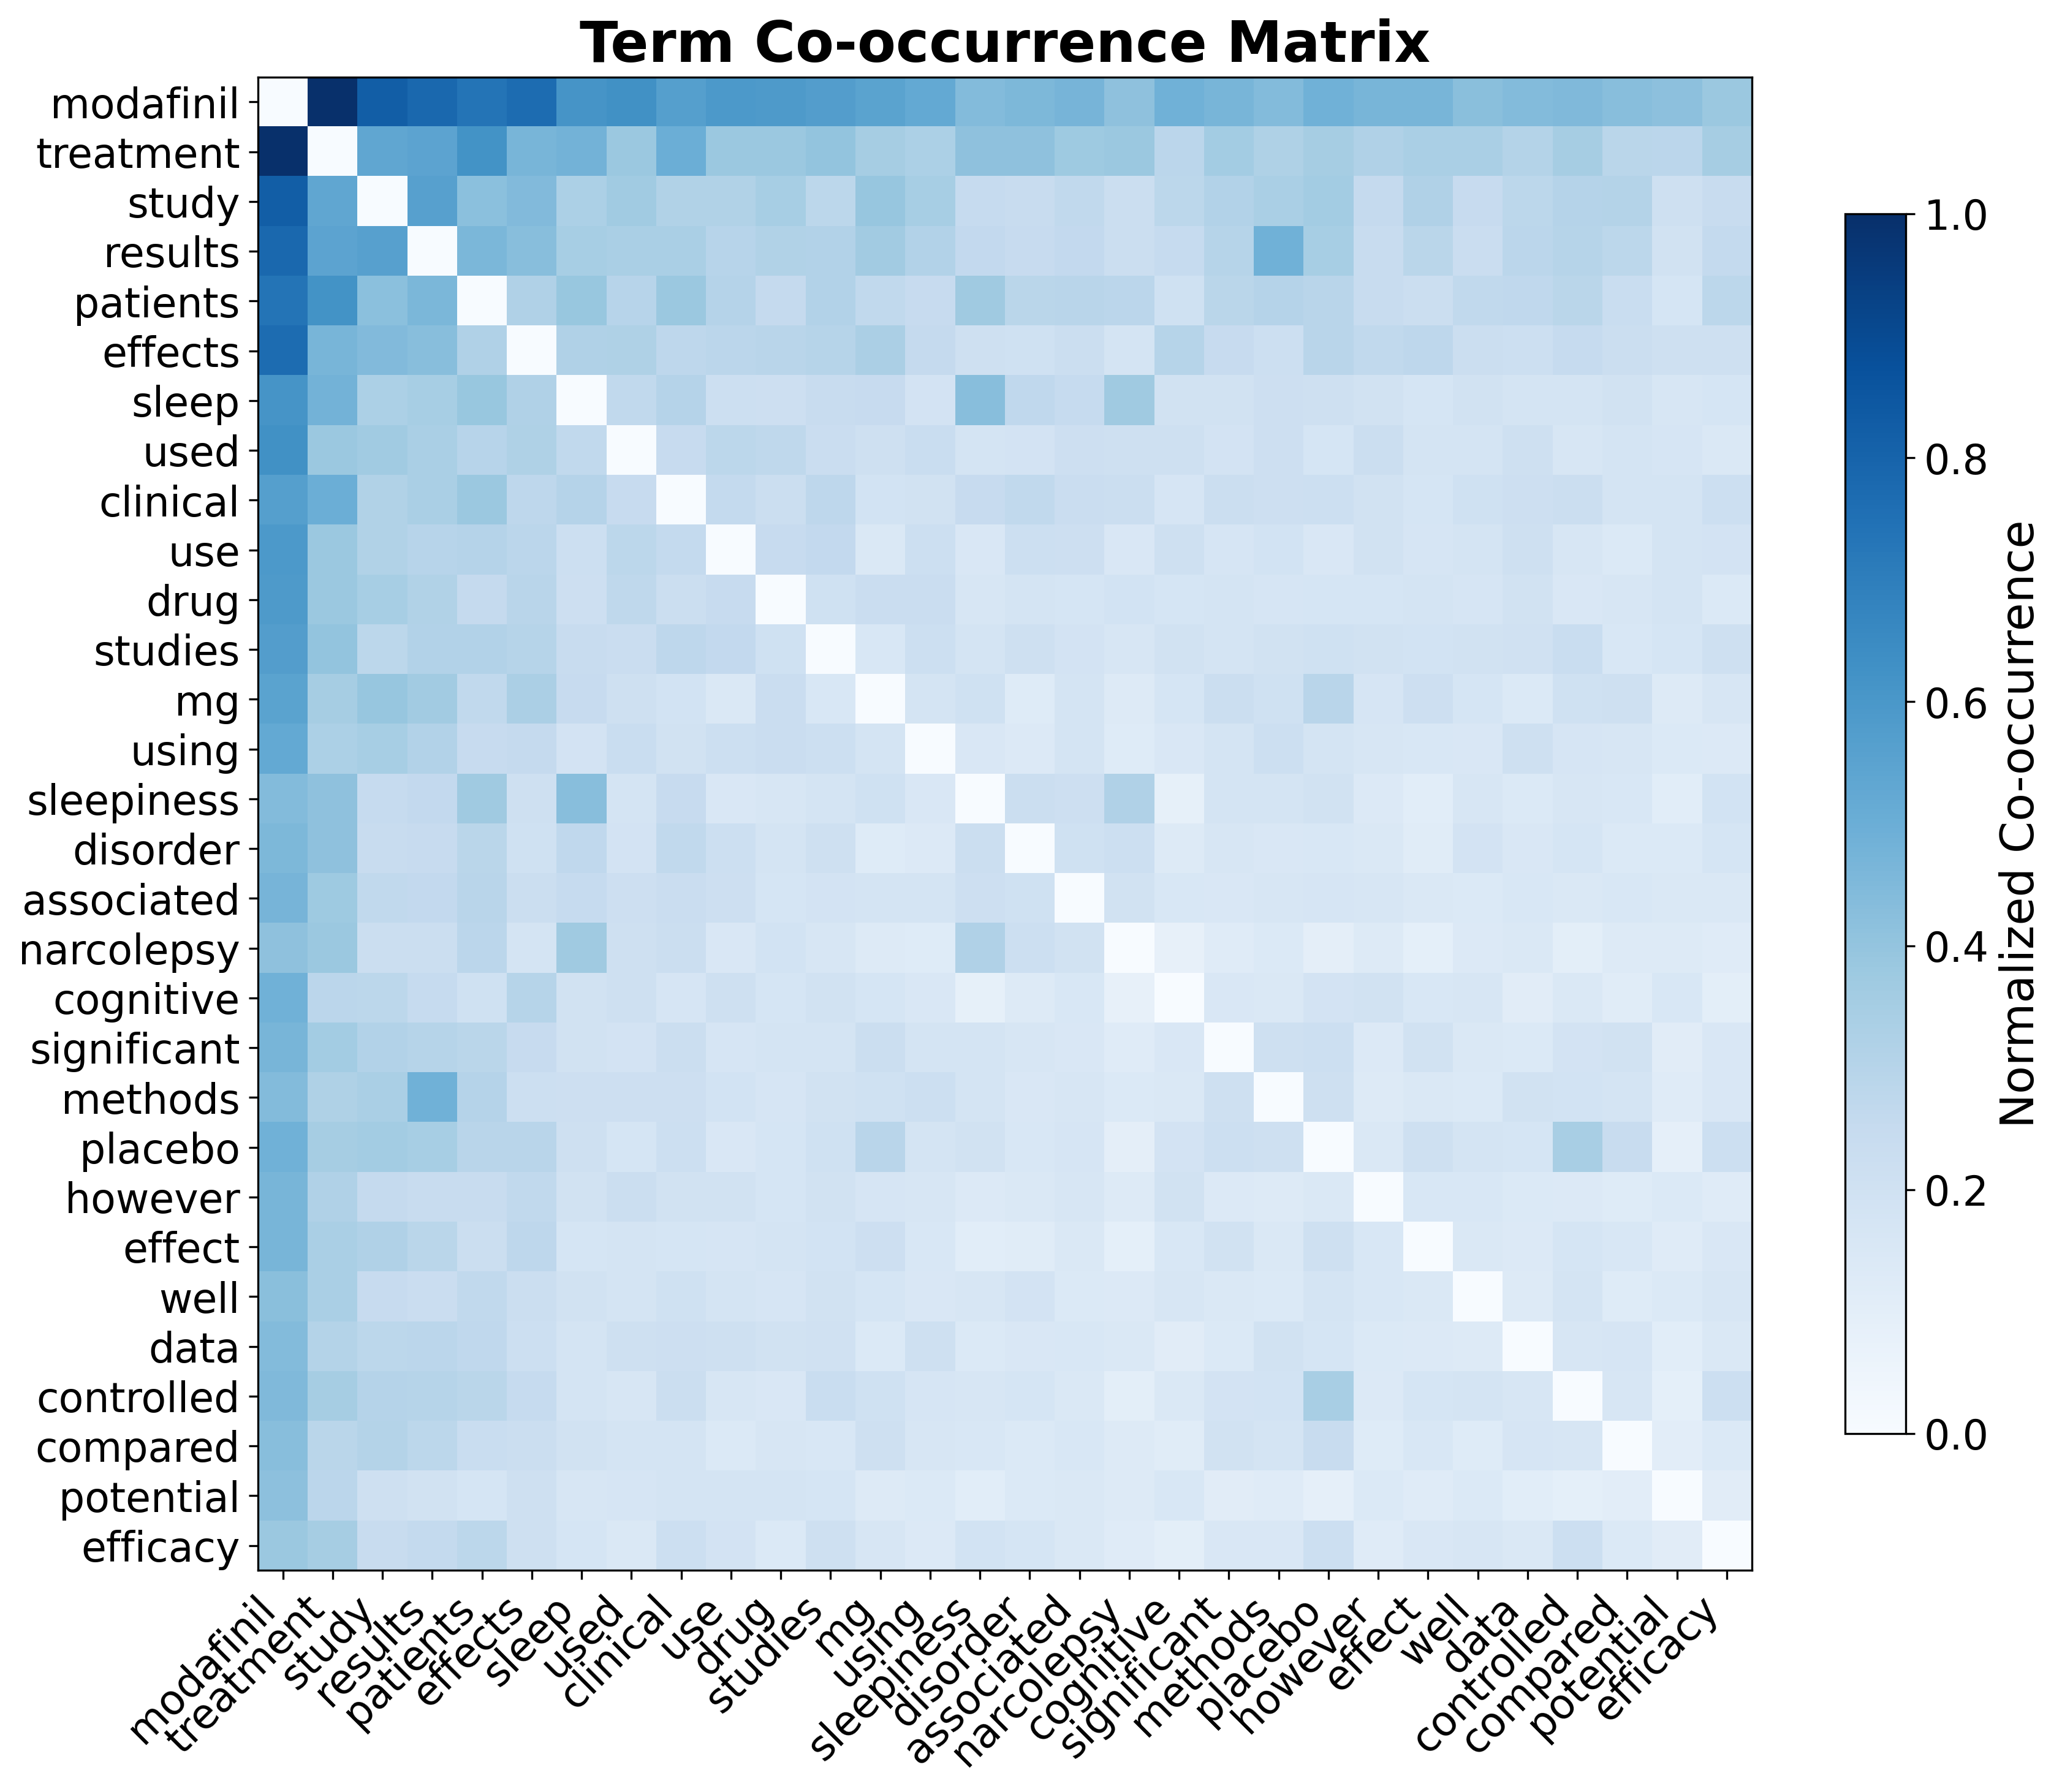
\includegraphics[keepaspectratio,alt={Term co-occurrence matrix for Modafinil. Each cell shows the normalized co-occurrence frequency of two terms within the same document, revealing which concepts tend to appear together in the literature.}]{../figures/cooccurrence_matrix.png}}\{\{\#fig:cooccurrence\_matrix\}\}

These embeddings support semantic retrieval over the corpus and the
visual map of the literature's topical geography.
\end{frame}

\end{document}
